%%%%%%%%%%%%%%%%%%%%%%%%%%%%%%%%%%%%%%%%%
% Journal Article
% LaTeX Template
% Version 1.3 (9/9/13)
%
% This template has been downloaded from:
% http://www.LaTeXTemplates.com
%
% Original author:
% Frits Wenneker (http://www.howtotex.com)
%
% License:
% CC BY-NC-SA 3.0 (http://creativecommons.org/licenses/by-nc-sa/3.0/)
%
%%%%%%%%%%%%%%%%%%%%%%%%%%%%%%%%%%%%%%%%%

%----------------------------------------------------------------------------------------
%	PACKAGES AND OTHER DOCUMENT CONFIGURATIONS
%----------------------------------------------------------------------------------------

\documentclass[twoside]{article}

\usepackage{lipsum} % Package to generate dummy text throughout this template

\usepackage[sc]{mathpazo} % Use the Palatino font
\usepackage[T1]{fontenc} % Use 8-bit encoding that has 256 glyphs
\linespread{1.05} % Line spacing - Palatino needs more space between lines
\usepackage{microtype} % Slightly tweak font spacing for aesthetics

\usepackage[hmarginratio=1:1,top=32mm,columnsep=20pt]{geometry} % Document margins
\usepackage{multicol} % Used for the two-column layout of the document
\usepackage[hang, small,labelfont=bf,up,textfont=it,up]{caption} % Custom captions under/above floats in tables or figures
\usepackage{booktabs} % Horizontal rules in tables
\usepackage{float} % Required for tables and figures in the multi-column environment - they need to be placed in specific locations with the [H] (e.g. \begin{table}[H])
\usepackage{hyperref} % For hyperlinks in the PDF
\usepackage{graphicx}
\usepackage{lettrine} % The lettrine is the first enlarged letter at the beginning of the text
\usepackage{paralist} % Used for the compactitem environment which makes bullet points with less space between them

\usepackage{abstract} % Allows abstract customization
\renewcommand{\abstractnamefont}{\normalfont\bfseries} % Set the "Abstract" text to bold
\renewcommand{\abstracttextfont}{\normalfont\small\itshape} % Set the abstract itself to small italic text

\usepackage{titlesec} % Allows customization of titles
\renewcommand\thesection{\Roman{section}} % Roman numerals for the sections
\renewcommand\thesubsection{\Roman{subsection}} % Roman numerals for subsections
\titleformat{\section}[block]{\large\scshape\centering}{\thesection.}{1em}{} % Change the look of the section titles
\titleformat{\subsection}[block]{\large}{\thesubsection.}{1em}{} % Change the look of the section titles

\usepackage{fancyhdr} % Headers and footers
\pagestyle{fancy} % All pages have headers and footers
\fancyhead{} % Blank out the default header
\fancyfoot{} % Blank out the default footer
\fancyhead[C]{MiNI - CIBA $\bullet$ November 2015} % Custom header text
\fancyfoot[RO,LE]{\thepage} % Custom footer text

%----------------------------------------------------------------------------------------
%	TITLE SECTION
%----------------------------------------------------------------------------------------

\title{\vspace{-15mm}\fontsize{24pt}{10pt}\selectfont\textbf{High Frequency Trading Price Prediction using LSTM Recursive Neural Networks}} % Article title

\author{
\large
\thanks{Project for Computational Intelligence Business Applications Course}\\[2mm] % Your name
\textsc{Karol Dzitkowski}\\
\normalsize \href{mailto:k.dzitkowski@gmail.com}{k.dzitkowski@gmail.com} \\
\normalsize Warsaw University of Technology\\
\vspace{-5mm}
}
\date{}

%----------------------------------------------------------------------------------------

\begin{document}

\maketitle % Insert title

\thispagestyle{fancy} % All pages have headers and footers

%----------------------------------------------------------------------------------------
%	ABSTRACT
%----------------------------------------------------------------------------------------

\begin{abstract}

The Recurrent Neural Network (RNN) is an extremely powerful model for problems in machine learning that require identifying complex dependencies between temporally distant inputs. It is often used in solving NLP problems, therefore it can be suitable also for stock market prediction. 
In this work I will try to use recurrent neural network with long short term memory to predict prices in high frequency stock exchange. This paper will show results of implementing such a solution on data from NYSE OpenBook history which allows to recreate the limit order book for any given time.

\end{abstract}

%----------------------------------------------------------------------------------------
%	ARTICLE CONTENTS
%----------------------------------------------------------------------------------------

\begin{multicols}{2} % Two-column layout throughout the main article text

\section{Introduction}

\lettrine[nindent=0em,lines=3]{L} ong Short Memory RNN architecture has been proved to be suprisingly successive in sequence prediction
resolving a problem with vanishing and exploding gradients. In this work I will use Hochreiter \& Schmidhuber (1997) version of LSTM layer. 
The Long Short-Term Memory (LSTM) is a specific RNN architecture whose design makes it much easier to train. While wildly successful in practice, the LSTM's architecture appears to be ad-hoc so it is not clear if it is optimal, and the significance of its individual components is unclear - which was checked by Google in [1]. The aim of this work is to see if the solution will be suitable for predicting prices in stock markets, which are one of the most difficult time series to predict.
Basing on time series data from NYSE OpenBook (which includes every ask and bid prices for one day)
I will try to predict next bid or ask value. If there exist any long or short term dependency with historical data, my LSTM model should outperform
basic perceptron which will be used for comparison. I will also check if changing LSTM model to GRU (Gated Recurrent Unit - Cho et al. 2014.) will
decrease an error rate to establish which solution is best.
All technical implementation will be done in Python using Keras [2] library based on Theano. For performance reasons most computations will be done on GPU using NVIDIA CUDA 7.5 technology. 


%------------------------------------------------

\section{Used method}

In order to gain some persistent knowledge in the network people invented Recurrent Neural Networks which address this issue.
They are networks with loops inside them, allowing information to persist. In that way they are able to learn some long term dependencies between
data in several time points. Usually we consider an unrolled RNN with some length creating chain-like structure.

\begin{figure}[H]
\centering
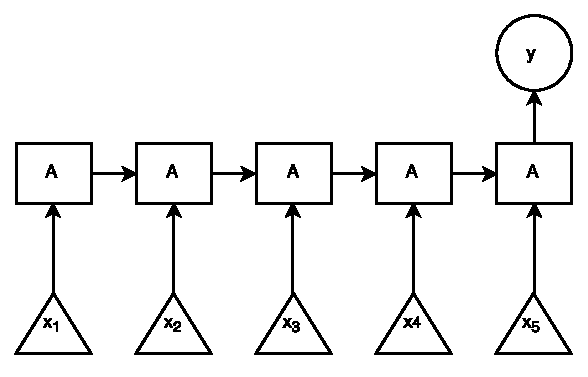
\includegraphics[scale=0.75]{RNN}
\caption{Recursive Neural Network}
\label{ref:rnn}
\end{figure} 

This way they seem to be related to sequences or lists, therefore it will be natural architecture of a network for all time series.
In a normal, basic version the hidden layer \emph{A} is just single \emph{sigmoid} or \emph{tanh} layer.  Due to the fact that for
learning such an architecture uses Backpropagation Through Time (BPTT) it is usually very difficult to train such networks. The problem
is known as vanishing and exploding gradient which makes it impossible for the network to learn long term dependencies. It is solved
by using Long Short Term Memory Networks (LSTM) that handles layer \emph{A} differently. In that model \emph{A} is more complex
structure containing several \emph{tanh} and \emph{sigmoid} layers and \emph{+}, \emph{*} operators.

\begin{figure}[H]
\centering
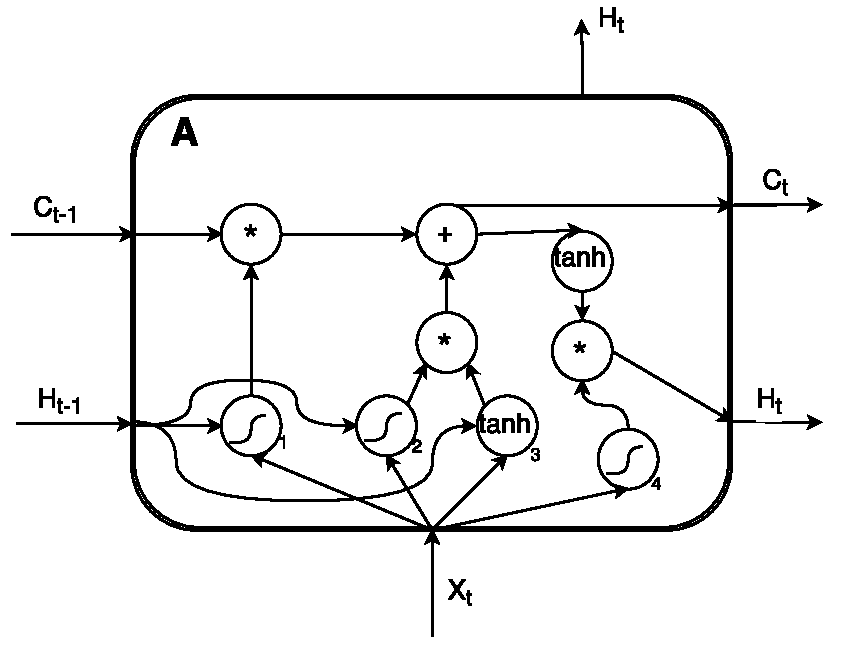
\includegraphics[scale=0.5]{LSTM}
\caption{Recursive Neural Network}
\label{ref:rnn}
\end{figure} 

LSTM handles and passes something called the cell state. It can add or remove information to/from the cell and in that way he stores
historical data. Mathematical definition of that architecture is shown below, where $x_{t}$ is our input, $H_{t-1}$ is the previous output and 
$W_{m}$ are the weights in layer m: \\
\newline
$ \alpha_{t} = \sigma(W_{1} * x_{t} + W_{1} * H_{t-1} + b_{1}) $ \\
$ \beta_{t} = \sigma(W_{2} * x_{t} + W_{2} * H_{t-1} + b_{2}) $ \\
$ \gamma_{t} = tanh(W_{3} * x_{t} + W_{3} * H_{t-1} + b_{3}) $ \\
$ \theta_{t} = \sigma(W_{4} * x_{t} + W_{4} * H_{t-1} + b_{4}) $ \\
\newline
then the new cell state and output are:  \\
\newline
$ C_{t} = \alpha_{t} * C_{t-1} + \beta_{t} * \gamma_{t} $ \\
$ H_{t} = \theta_{t} * tanh(C_{t}) $ \\


Data from NYSE contains information about the symbol of stock, event type, price and volume as well as very precise time to microseconds.
Each record is either bid or ask wchich is indicated by \emph(Side) field of the data.  

\begin{table}[H]
\caption{Selected TAQ NYSE OpenBook Fields}
\centering
\begin{tabular}{ll}
Symbol & Char(11) \\
TradingStatus & Char(1) \\
SourceTime & Int(4) \\
SourceTimeMicroSecs & Int(2) \\
PriceScaleCode & Int(1) \\
PriceNumerator & Int(4) \\
Volume & Int(4) \\ 
Side & Char(1) \\
\end{tabular}
\end{table}

For me the most important are price, volume na side data, because I will use them among others as an input to the network. 
Network will be always trained only for one symbol and for events of submission. I am going to experiment with different inputs,
probably using some feature extraction, or choosing custom subset of features by myself.
Inputs I am going to consider are:

\begin{itemize}
\item Time - Time since last ask or bid
\item Price - Ask or bid price
\item MidPrice - Difference between highest bid and lowest ask price divided by 2
\item Volume - Volume of last ask or bid
\item Side - Boolean indicating if it was bid or ask
\item PriceDiff - Difference of price between last bid or ask
\end{itemize}

The same inputs will be used to learn ordinary perceptron with one hidden layer. Number of nodes in the hidden layer in that \emph(testing)
perceptron will be optimized to maximize its performance. The output for both neural networks will be the next bid or ask price which should
appear in the book. \\
\newline
For the estimation of performance of my neural networks I will use mean squared error loss function: \\
\newline
\begin{center}
$ err(t) = \frac{\sum\limits_{i=1}^t (y_{i} - Y_{i})}{t - 1} $
\end{center}
%------------------------------------------------

\section{Implementation details}

Keras library will be used for development of the solution, since it provides all necessary layer types including LSTM in the version described
above as well as GRU. Since it uses Theano under the hood it is possible to swich on GPU usage, involving that time consuming computations
will be executed on my NVIDIA graphic card using CUDA technology.

%------------------------------------------------

\section{Results}

\section{Conclusion}

%----------------------------------------------------------------------------------------
%	REFERENCE LIST
%----------------------------------------------------------------------------------------

\begin{thebibliography}{99} % Bibliography - this is intentionally simple in this template

\bibitem{tut01}
    ``LSTM implementation explained'' - \emph{https://apaszke.github.io/lstm-explained.html} Adam Paszke, 30 Aug 2015
\bibitem{tut02}
    ``Recurrent Neural Networks Tutorial - Implementing a RNN with Python, Numpy and Theano'' - \emph{http://www.wildml.com/2015/09/recurrent-neural-networks-tutorial-part-2-implementing-a-language-model-rnn-with-python-numpy-and-theano/}
\bibitem{tut03}
    ``Keras library'' - \emph{http://keras.io}
\bibitem{tut04}
    ``Supervised Sequence Labelling with Recurrent Neural Networks'' - \emph{http://www.cs.toronto.edu/~graves/preprint.pdf} Alex Graves
\end{thebibliography}

%----------------------------------------------------------------------------------------

\end{multicols}

\end{document}
